\textbf{A continuación, se muestran tres representaciones posibles referidas a las relaciones entre Materias, Profesores y Alumnos. Analiza las ventajas y desventajas de cada propuesta, contestando las preguntas que se presentan a continuación:}

\begin{center}
    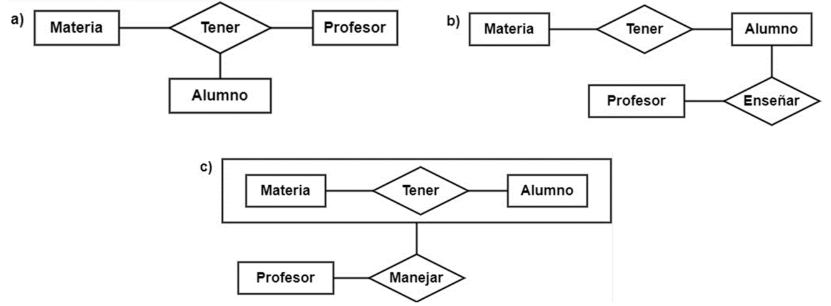
\includegraphics[width=16cm]{resources/ER_2.1.png}
\end{center}

Indica qué diagramas representan la información requerida por las siguientes solicitudes de información:

\begin{enumerate}
    \item \textbf{¿A qué alumnos imparte clases el profesor Carlos Sánchez en la materia Bases de Datos?} \\

    Como dice la pregunta hay 3 relaciones, entonces debemos identificar la relación entre Profesor, Materia y Alumno. \\

    Por lo que el diagrama \textbf{$"b"$} es el más adecuado; pues como se puede ver incluye una relación directa de \textbf{Enseñar} entre \textbf{Profesor} y \textbf{Alumno}, lo cual nos permite conocer a qué \textbf{Alumnos} enseña el profesor en una \textbf{Materia} específica. \\

    \item \textbf{¿Qué materias imparte la profesora Patricia Ríos?} \\

    Como dice la pregunta, requerimos identificar la relación entre \textbf{Profesor} y \textbf{Materia}. \\

    Por lo que el diagrama \textbf{$"a"$} es el más adecuado; pues como se puede ver hay una relación \textbf{Tener} entre \textbf{Profesor} y \textbf{Materia} que esta directamente representada, y esto nos permite conocer qué materias tiene a su cargo la profesora Patrícia Ríos. \\
    
    \item \textbf{¿Qué alumnos están inscritos en la materia Ingeniería de Software?} \\

    Para esta pregunta, el diagrama \textbf{$"a"$} también es útil, ya que la relación entre \textbf{Materia} y \textbf{Alumno} está directamente representada. Esto permite saber qué \textbf{alumnos} están relacionados con la \textbf{materia} Ingeniería de Software.
    
\end{enumerate}
